% (c) 2012-2013 Claudio Carboncini - claudio.carboncini@gmail.com
% (c) 2012-2014 Dimitrios Vrettos - d.vrettos@gmail.com

\chapter{Equazioni}

\section{Equazioni di grado superiore al primo riducibili al primo grado}

Nel capitolo \ref{cap:equazioni_I_grado} abbiamo affrontato le equazioni di primo grado. Adesso consideriamo le equazioni di grado superiore al primo che possono essere ricondotte ad equazioni di primo grado,
utilizzando la legge di annullamento del prodotto (legge \ref{legge:annullamento_del_prodotto} a pagina \pageref{legge:annullamento_del_prodotto}).

\begin{exrig}
 \begin{esempio}
Risolvere~$x^{2}-4=0$.

Il polinomio al primo membro può essere scomposto in fattori:~$(x-2)(x+2)=0$.
Per la legge di annullamento, il prodotto dei due binomi si annulla se~$x-2=0$ oppure se~$x+2=0$.
Di conseguenza si avranno le soluzioni:~$x=2$ e $x=-2$.
 \end{esempio}
\end{exrig}

In generale, se si ha un’equazione di grado~$n$ scritta in forma normale~$P(x)=0$ e se il polinomio~$P(x)$ è
fattorizzabile nel prodotto di~$n$ fattori di primo grado:
\begin{equation*}
(x-a_{1})(x-a_{2})(x-a_{3})\ldots (x-a_{n-1})(x-a_{n})=0
\end{equation*}
applicando la legge di annullamento del prodotto, le soluzioni dell’equazione si ottengono determinando le soluzioni delle singole~$n$
equazioni di primo grado, cioè risolvendo:
\begin{equation*}
x-a_{1}=0\text{,~~~}x-a_{2}=0\text{,~~~}x-a_{3}=0\text{,~~~}\ldots\text{,~~~}x-a_{n-1}=0\text{,~~~}x-a_{n}=0.
\end{equation*}
Pertanto l’insieme delle soluzioni dell’equazione data sarà:~$\IS=\{a_{1}\text{,~}a_{2}\text{,~}a_{3}\text{,~}\ldots\text{,~}a_{n-1}\text{,~}a_{n}\}$.

\begin{exrig}
 \begin{esempio}
Risolvere~$x^{2}-x-2=0$.

Scomponendo in fattori il polinomio al primo membro, ricercando quei due numeri la cui somma è pari a~$-1$ e il cui prodotto è pari a~$-2$, 
si ha:~$(x+1)(x-2)=0$.
Utilizzando la legge di annullamento del prodotto, si ottiene il seguente insieme di soluzioni:~$\IS=\{-1\text{,~}2\}$.
 \end{esempio}

 \begin{esempio}
Risolvere~$x^{4}-5x^{2}+4=0$.

Scomponendo in fattori il polinomio al primo membro, utilizzando la regola della scomposizione del particolare trinomio di secondo grado,
si ottiene:~$(x^{2}-1)(x^{2}-4)=0$. Scomponendo ulteriormente in fattori si ha:
\begin{equation*}
(x-1)(x+1)(x-2)(x+2)=0.
\end{equation*}
Per la legge di annullamento del prodotto è necessario risolvere le equazioni:
\begin{equation*}
x-1=0\: \Rightarrow\: x=1\text{,}\quad x+1=0\: \Rightarrow\: x=-1\text{,}\quad x-2=0\: \Rightarrow\: x=2\text{,}\quad x+2=0\: \Rightarrow\: x=-2.
\end{equation*}
L’insieme delle soluzioni:~$\IS=\{+1\text{,~}-1\text{,~}+2\text{,~}-2\}$.
 \end{esempio}

\end{exrig}

\ovalbox{\risolvii \ref{ese:20.1}, \ref{ese:20.2}, \ref{ese:20.3}, \ref{ese:20.4}, \ref{ese:20.5}, \ref{ese:20.6}, \ref{ese:20.7}, \ref{ese:20.8},
\ref{ese:20.9}, \ref{ese:20.10}}

\vspazio\ovalbox{\ref{ese:20.11}, \ref{ese:20.12}, \ref{ese:20.13}}

\section{Equazioni numeriche frazionarie}

Affrontiamo ora le equazioni in cui l'incognita compare anche al denominatore.

\begin{definizione} Un’equazione in cui l’incognita compare al denominatore si chiama \emph{frazionaria} o \emph{fratta}.
\end{definizione}

\begin{exrig}
 \begin{esempio}
Risolvere~$\dfrac{3x-2}{1+x}=\dfrac{3x}{x-2}$.
 \end{esempio}
Questa equazione si differenzia da quelle affrontate in precedenza per il fatto che l'incognita compare anche al denominatore.
Riflettendo sulla richiesta del problema, possiamo senz’altro affermare che, se esiste il valore che rende
la frazione al primo membro uguale alla frazione al secondo membro, esso non deve annullare nessuno dei due denominatori,
poiché in questo caso renderebbe priva di significato la scrittura, in quanto frazioni con denominatore~$0$ sono prive di significato.

Per risolvere un'equazione frazionaria, prima di tutto dobbiamo renderla nella forma
\begin{equation*}
\frac{F(x)}{G(x)}=0.
\end{equation*}

\begin{enumeratea}
 \item Determiniamo il~$\mcm$ dei denominatori, $\mcm=(1+x)\cdot (x-2)$.
    Osserviamo che per~$x = -1$ oppure per~$x = 2$ le frazioni perdono di significato, in quanto si annulla il denominatore;
 \item imponiamo le condizioni di esistenza:~$1+x\neq~0$ e~$x-2\neq~0$ cioè~$\CE x\neq -1\wedge x\neq~2$. La ricerca dei valori
    che risolvono l'equazione viene ristretta all'insieme~$\Dom=\insR-\{-1\text{,~}2\}$, detto \emph{dominio} dell’equazione o
    \emph{insieme di definizione};
 \item applichiamo il primo principio d’equivalenza trasportando al primo membro la frazione che si trova al secondo membro
    e riduciamo allo stesso denominatore ($\mcm$)
    \begin{equation*}
      \frac{(3x-2)\cdot (x-2)-3x\cdot (1+x)}{(1+x)\cdot (x-2)}=0;
    \end{equation*}
 \item applichiamo il secondo principio di equivalenza moltiplicando ambo i membri per il~$\mcm$,
    certamente diverso da zero per le condizioni poste precedentemente. L’equazione diventa:~$(3x-2)\cdot (x-2)-3x\cdot (1+x)=0$;
 \item eseguiamo le moltiplicazioni e sommiamo i monomi simili per portare l’equazione alla forma canonica:
    $3x^{2}-6x-2x+4-3x-3x^{2}=0\: \Rightarrow\: -11x=-4$;
 \item dividiamo ambo i membri per~$-11$, per il secondo principio di equivalenza si ha:~$x=\frac{4}{11}$;
 \item confrontiamo il valore trovato con le~$\CE$: in questo caso la soluzione appartiene al dominio~$\Dom$, quindi possiamo concludere
    che è accettabile. L’insieme soluzione è:~$\IS=\left\{\frac{4}{11}\right\}$.
\end{enumeratea}

%\newpage
 \begin{esempio}
Risolvere~$\dfrac{x^{2}+x-3}{x^{2}-x}=1-\dfrac{5}{2x}$.
\end{esempio}

\begin{enumeratea}
 \item Determiniamo il~$\mcm$ dei denominatori. Per fare questo dobbiamo prima scomporli in fattori.
    Riscriviamo:~$\dfrac{x^{2}+x-3}{x\cdot (x-1)}=1-\dfrac{5}{2x}$ con~$\mcm=2x\cdot (x-1)$;
 \item condizioni di esistenza: \[x-1\neq~0\wedge~2x\neq~0\text{,}\] cioè~$x\neq~1\wedge x\neq~0$. Il dominio è~$\Dom=\insR-\{1\text{,~}0\}$;
 \item trasportiamo al primo membro ed uguagliamo a zero \[\frac{x^{2}+x-3}{x\cdot (x-1)}-1+\frac{5}{2x}=0\]
    e riduciamo allo stesso denominatore ($\mcm$) ambo i membri \[\frac{2x^{2}+2x-6-2x^{2}+2x+5x-5}{2x\cdot (x-1)}=0;\]
 \item applichiamo il secondo principio di equivalenza moltiplicando ambo i membri per il~$\mcm$,
    certamente diverso da zero per le condizioni poste in precedenza. L’equazione diventa:~$2x^{2}+2x-6-2x^{2}+2x+5x-5=0$;
 \item riduciamo i monomi simili per portare l’equazione alla forma canonica:~$9x=11$;
 \item dividiamo ambo i membri per~$9$, otteniamo:~$x=\frac{11}{9}$;
 \item confrontando con le~$\CE$, la soluzione appartiene all’insieme~$\Dom$, dunque è accettabile e l’insieme soluzione è:
    $\IS=\left\{\frac{11}{9}\right\}$.
\end{enumeratea}

\end{exrig}

\ovalbox{\risolvii \ref{ese:20.15}, \ref{ese:20.16}, \ref{ese:20.17}, \ref{ese:20.18}, \ref{ese:20.19}, \ref{ese:20.20}, \ref{ese:20.21},
\ref{ese:20.22}, \ref{ese:20.23}, \ref{ese:20.24}, \ref{ese:20.25}}

\vspazio\ovalbox{\ref{ese:20.26}, \ref{ese:20.27}}

\section{Equazioni letterali}
Quando si risolvono problemi, ci si ritrova a dover tradurre nel linguaggio simbolico delle proposizioni del tipo:
<<Un lato di un triangolo scaleno ha lunghezza pari a~$k$ volte la lunghezza dell’altro e la loro somma è pari a~$2k$>>.
Poiché la lunghezza del lato del triangolo non è nota, ad essa si attribuisce il valore incognito~$x$ e quindi la proposizione
viene tradotta dalla seguente equazione:~$x+kx=2k$.

È possibile notare che i coefficienti dell’equazione non sono solamente numerici, ma contengono una lettera dell’alfabeto diversa
dall’incognita. Qual è il ruolo della lettera~$k$?
Essa prende il nome di \emph{parametro} ed è una costante che rappresenta dei numeri fissi, quindi, può assumere dei valori prefissati.
Ogni volta che viene fissato un valore di~$k$, l’equazione precedente assume una diversa forma. Infatti si ha:
\begin{center}
\begin{tabular}{cl}
\toprule
Valore di~$k$ & Equazione corrispondente\\
\midrule
$0$ & $x=0$\\
$2$ & $x+2x=4$\\
$-\frac{1}{2}$ & $x-\frac{1}{2}x=-1$\\
\bottomrule
\end{tabular}
\end{center}

Si può quindi dedurre che il parametro diventa una costante, all’interno dell’equazione nell’incognita~$x$, ogni volta che se ne sceglie il valore.

Si supponga che il parametro~$k$ assuma valori all’interno dell’insieme dei numeri reali. Lo scopo è quello di risolvere l’equazione,
facendo attenzione a rispettare le condizioni che permettono l’uso dei principi d’equivalenza e che permettono di ridurla in forma normale.

Riprendiamo l'equazione  $x+kx=2k$, raccogliamo a fattore comune la~$x$ si ha:
\begin{equation*}
 (k+1)x=2k.
\end{equation*}
Per determinare la soluzione di questa equazione di primo grado, è necessario utilizzare il secondo principio d’equivalenza e
dividere ambo i membri per il coefficiente~$k+1$.
Si ricordi però che il secondo principio ci permette di moltiplicare o dividere i due membri dell'equazione per una stessa espressione,
purché questa sia diversa da zero.
Per questa ragione, nella risoluzione dell’equazione~$(k+1)x=2k$ è necessario distinguere i due casi:
\begin{itemize*}
\item se~$k+1\neq~0$, cioè se~$k\neq -1$, è possibile dividere per~$k+1$ e si ha~$x=\dfrac{2k}{k+1}$;
\item se~$k+1=0$, cioè se~$k=-1$, sostituendo tale valore all'equazione si ottiene l’equazione~$(-1+1)x=2\cdot (-1)$,
   cioè~$0\cdot x=-2$ che risulta impossibile.
\end{itemize*}
Riassumendo si ha:
\begin{center}
\begin{tabular}{lcc}
\toprule
\multicolumn{3}{c} {$x+kx=2k$~~con~$k \in \insR$}\vspace{1.05ex}\\
Condizioni sul parametro & Soluzione & Equazione\\
\midrule
$k=-1$ & nessuna & impossibile \\
$k\neq-1$ & $x=\dfrac{2k}{k+1}$ & determinata \\
\bottomrule
\end{tabular}
\end{center}

Ritorniamo ora al problema sul triangolo, spesso nell’enunciato del problema sono presenti delle limitazioni implicite
che bisogna trovare. Infatti, dovendo essere~$x$ un lato del triangolo esso sarà un numero reale positivo.
Di conseguenza, dovendo essere l’altro lato uguale a~$k$ volte~$x$, il valore di~$k$ deve necessariamente essere anch'esso positivo, ovvero~$k>0$.
Di conseguenza il parametro~$k$ non può mai assumere il valore~$-1$ e quindi il problema geometrico ammette sempre una soluzione.

Questa analisi effettuata sui valori che può assumere il parametro~$k$, prende il nome di \emph{discussione dell’equazione}.
\begin{procedura}
Stabilire quando una equazione è determinata, indeterminata, impossibile.

In generale, data l'equazione~$ax+b=0$ si ha~$ax=-b$ e quindi:
\begin{enumeratea}
\item se~$a\neq~0$, l’equazione è determinata e ammette l’unica soluzione~$x=-\dfrac{b}{a}$;
\item se~$a=0$ e~$b\neq~0$, l’equazione è impossibile;
\item se~$a=0$ e~$b=0$, l’equazione è soddisfatta da tutti i valori reali di~$x$, ovvero è indeterminata.
\end{enumeratea}
\end{procedura}

\begin{exrig}
 \begin{esempio}
Risolvere e discutere~$1+x+m=(x+1)^{2}-x(x+m)$.

Dopo aver fatto i calcoli si ottiene l’equazione~$(m-1)\cdot x=-m$ e quindi si ha:
\begin{itemize*}
 \item Se~$m-1\neq~0$, cioè se~$m\neq~1$, è possibile dividere ambo i membri per~$m-1$ e si ottiene l’unica soluzione~$x=-{\dfrac{m}{m-1}}$;
 \item se~$m-1=0$, cioè se~$m=1$, sostituendo nell'equazione il valore~$1$ si ottiene~$0\cdot x=-1$, che risulta impossibile.
\end{itemize*}
 \end{esempio}

 \begin{esempio}
Risolvere e discutere~$(k+3)x=k+4x(k+1)$.

Effettuando i prodotti si ottiene l’equazione:~$(3k+1)x=-k$ e quindi si ha:
\begin{itemize*}
 \item Se~$3k+1\neq~0$, cioè se~$k\neq -{\frac{1}{3}}$, è possibile dividere ambo i membri per~$3k+1$ e si ottiene l’unica soluzione~$x=\dfrac{-k}{3k+1}$;
 \item se~$k=-{\frac{1}{3}}$, sostituendo questo valore di~$k$ nell'equazione si ottiene~$0\cdot x=\frac{1}{3}$, che risulta un'equazione impossibile.
\end{itemize*}
 \end{esempio}

 \begin{esempio}
Risolvere e discutere~$a^{2}\cdot x=a+1+x$.

Portiamo al primo membro tutti i monomi che contengono l'incognita~$a^{2}\cdot x-x=a+1$.
Raccogliamo a fattore comune l'incognita~$x\cdot \left(a^{2}-1\right)=a+1$.
Scomponendo in fattori si ha l'equazione~$x\cdot \left(a-1\right)\left(a+1\right)=a+1$.

I valori di~$a$ che annullano il coefficiente dell'incognita sono~$a=1$ e~$a=-1$.
\begin{itemize*}
 \item Se nell'equazione sostituisco~$a=1$, ottengo l'equazione~$0x=2$ che è impossibile;
 \item se sostituisco~$a=-1$, ottengo l'equazione~$0x=0$ che è indeterminata;
 \item escludendo i casi~$a=1$ e~$a=-1$, che annullano il coefficiente della~$x$, posso applicare il secondo principio
    di equivalenza delle equazioni e dividere primo e secondo membro per~$(a+1)(a-1)$, ottenendo~$x=\dfrac{a+1}{\left(a+1\right)\cdot \left(a-1\right)}=\dfrac{1}{a-1}$.
\end{itemize*}
 \end{esempio}
Ricapitolando:
se~$a=1$, allora~$\IS=\emptyset$; se~$a=-1$, allora~$\IS=\insR$; se~$a\neq +1\wedge a\neq -1$, allora~$\IS=\left\{\dfrac{1}{a-1}\right\}$.
\end{exrig}

\ovalbox{\risolvii \ref{ese:20.34}, \ref{ese:20.35}, \ref{ese:20.36}, \ref{ese:20.37}, \ref{ese:20.38}, \ref{ese:20.39}, \ref{ese:20.40}}

\subsection{Equazioni con due parametri}

\begin{exrig}
 \begin{esempio}
Risolvere e discutere~$(b+a)x-(b+2)(x+1)=-1$.

Mettiamo l'equazione in forma canonica:~$bx+ax-bx-b-2x-2=-1$.
Raccogliamo a fattore comune l'incognita~$(a-2)x=b+1$.
\begin{itemize*}
 \item Se~$a-2=0$ l'equazione è impossibile o indeterminata. In questo caso:
  \begin{itemize*}
   \item se~$b+1=0$ è indeterminata;
   \item se~$b+1\neq~0$ è impossibile;
  \end{itemize*}
 \item se~$a-2\neq~0$ l'equazione è determinata e la sua soluzione è~$x=\dfrac{b+1}{a-2}$.
\end{itemize*}
 \end{esempio}
Riassumendo:
se~$a=2\wedge b=-1$ allora~$\IS=\insR$; se~$a=2\wedge b\neq -1$ allora~$\IS=\emptyset$; se~$a\neq~2\wedge b\neq -1$ allora~$\IS=\left\{\dfrac{b+1}{a-2}\right\}$.
\end{exrig}

\ovalbox{\risolvii \ref{ese:20.41}, \ref{ese:20.42}, \ref{ese:20.43}}

\subsection{Equazioni letterali, caso in cui il denominatore contiene il parametro}

\begin{exrig}
 \begin{esempio}
Risolvere e discutere~$\dfrac{x+a}{2a-1}-\dfrac{1}{a-2a^{2}}=\dfrac{x}{a}$ con~$a\in \insR$.

Questa equazione è intera, pur presentando termini frazionari.
Sappiamo che ogni volta che viene fissato un valore per il parametro, l’equazione assume una forma diversa;
la presenza del parametro al denominatore ci obbliga ad escludere dall’insieme dei numeri reali quei valori che annullano il denominatore.

Per~$a=0\vee a=\frac{1}{2}$ si annullano i denominatori, quindi l’equazione è priva di significato.
Per risolvere l’equazione abbiamo bisogno delle condizioni di esistenza~$\CE a\neq~0$ e $a\neq \frac{1}{2}$.

Procediamo nella risoluzione, riduciamo allo stesso denominatore ambo i membri dell’equazione:
$\dfrac{a\cdot (x+a)+1}{a\cdot (2a-1)}=\dfrac{x\cdot (2a-1)}{a\cdot (2a-1)}$.
Applichiamo il secondo principio moltiplicando ambo i membri per il~$\mcm$, otteniamo:~$ax+a^{2}+1=2ax-x$
che in forma canonica è
\begin{equation*}
 x\cdot (a-1)=a^{2}+1.
\end{equation*}

Il coefficiente dell’incognita dipende dal valore assegnato al parametro $a$; procediamo quindi alla discussione:
\begin{itemize*}
 \item se~$a-1\neq~0$ cioè~$a\neq~1$ possiamo applicare il secondo principio e dividere ambo i membri per il coefficiente
    $a-1$ ottenendo~$x=\dfrac{a^{2}+1}{a-1}$. L’equazione è determinata:
    \[\IS=\left\{\frac{a^{2}+1}{a-1}\right\};\]
 \item se~$a-1=0$ cioè~$a=1$ l’equazione diventa~$0\cdot x=2$. L’equazione è impossibile:~$\IS=\emptyset$.
\end{itemize*}

Riassumendo si ha:
\begin{center}
\begin{tabular}{lll}
\toprule
\multicolumn{3}{c} {$\frac{x+a}{2a-1}-\frac{1}{a-2a^{2}}=\frac{x}{a}$~~con~$a\in \insR$}\vspace{1.05ex}\\
Condizioni sul parametro & Insieme Soluzione & Equazione\\
\midrule
$a=0\vee a=\frac{1}{2}$ & & priva di significato\\
$a=1$ & $\IS=\emptyset$ & impossibile \\
$a\neq~0\wedge a\neq \frac{1}{2}\wedge a\neq~1$ & $\IS=\left\{\frac{a^{2}+1}{a-1}\right\}$ & determinata \\
\bottomrule
\end{tabular}
\end{center}
 \end{esempio}

 \begin{esempio}
Risolvere e discutere~$\dfrac{a-x}{a-2}+\dfrac{2ax}{a^{2}-4}-\dfrac{2-x}{a+2}=0$ con~$a\in \insR$.

Scomponendo i denominatori troviamo il~$\mcm=a^2-4$.
Pertanto se~$a=2$ o~$a=-2$ il denominatore si annulla e quindi l’equazione è priva di significato.
Per poter procedere nella risoluzione poni le~$\CE a\neq -2\wedge a\neq~2$.

Riducendo allo stesso denominatore:~$\dfrac{(a-x)(a+2)+2ax-(2-x)(a-2)}{(a+2)(a-2)}=0$.

Applica il secondo principio per eliminare il denominatore e svolgi i calcoli. Arrivi alla forma canonica che è
 $2\cdot (a-2)\cdot x=a^{2}+4$.

Per le~$\CE$ sul parametro, il coefficiente dell’incognita è sempre diverso da zero, pertanto puoi dividere per~$2(a-2)$ e ottieni
$x=\dfrac{a^{2}+4}{2(a-2)}$.

Riassumendo si ha:
\begin{center}
\begin{tabular}{lll}
\toprule
\multicolumn{3}{c} {$\frac{a-x}{a-2}+\frac{2ax}{a^{2}-4}-\frac{2-x}{a+2}=0$ con~$a\in \insR$}\vspace{1.05ex}\\
Condizioni sul parametro & Insieme Soluzione & Equazione\\
\midrule
$a=-2\vee a=+2$ & & priva di significato\\
$a\neq -2\wedge a\neq +2$ & $\IS=\left\{\frac{a^{2}+4}{2(a-2)}\right\}$ & determinata \\
\bottomrule
\end{tabular}
\end{center}
 \end{esempio}
\end{exrig}

\subsection{Equazioni letterali frazionarie}

\subsubsection{Caso in cui il denominatore contiene solo l’incognita}

\begin{exrig}
 \begin{esempio}
Risolvere e discutere~$\dfrac{x+4a}{3x}=a-\dfrac{2x+2a}{6x}$ con~$a\in \insR$.

Questa equazione è frazionaria o fratta perché nel denominatore compare l’incognita.
Sappiamo che risolvere un’equazione significa determinare i valori che, sostituiti all’incognita, rendono vera
l’uguaglianza tra il primo e il secondo membro. Non sappiamo determinare tale valore solamente analizzando l’equazione,
ma certamente possiamo dire che non dovrà essere~$x = 0$ perché tale valore, annullando i denominatori, rende privi di
significato entrambi i membri dell’equazione.

Poniamo allora una condizione sull’incognita: la soluzione è accettabile se~$x\neq~0$.
Non abbiamo invece nessuna condizione sul parametro.

Procediamo quindi con la riduzione allo stesso denominatore di ambo i membri dell’equazione
$\dfrac{2x+8a}{6x}=\dfrac{6ax-2x-2a}{6x}$; eliminiamo il denominatore che per la condizione posta è diverso da zero.
Eseguiamo i calcoli al numeratore e otteniamo~$4x-6ax=-10a$ da cui la forma canonica:
\begin{equation*}
 x\cdot (3a-2)=5a.
\end{equation*}

Il coefficiente dell’incognita contiene il parametro, quindi procediamo alla discussione:
\begin{enumeratea}
 \item se~$3a-2\neq~0$ cioè~$a\neq \frac{2}{3}$ possiamo applicare il secondo principio e dividere ambo i membri per il coefficiente
      $3a-2$ ottenendo~$x=\frac{5a}{3a-2}$. L’equazione è determinata:~$\IS=\left\{\frac{5a}{3a-2}\right\}$.
      A questo punto dobbiamo ricordare la condizione sull'incognita, cioè~$x\neq~0$,
      quindi la soluzione è accettabile se~$x=\frac{5a}{3a-2}\neq~0 \Rightarrow a\neq~0$;
 \item se~$3a-2=0$ cioè~$a=\frac{2}{3}$ l’equazione diventa~$0\cdot x=\frac{10}{3}$, cioè l’equazione è impossibile:~$\IS=\emptyset$.
\end{enumeratea}
Riassumendo si ha la tabella:
\begin{center}
\begin{tabular}{llll}
\toprule
\multicolumn{4}{c} {$\dfrac{x+4a}{3x}=a-\dfrac{2x+2a}{6x}$ con~$a\in \insR$}\vspace{1.05ex}\\
\multicolumn{2}{c}{Condizioni} & &\\
parametro & incognita & Insieme Soluzione & Equazione\\
\midrule
 &$x\neq0$ & & \\
$a=\frac{2}{3}$ & & $\IS=\emptyset$ & impossibile \\
$a\neq\frac{2}{3}$ & & $\IS=\left\{\frac{5a}{3a-2}\right\}$ & determinata \\
$a\neq \frac{2}{3}\wedge a\neq0$ & accettabile &$x=\frac{5a}{3a-2}$ & \\
\bottomrule
\end{tabular}
\end{center}
 \end{esempio}
\end{exrig}

\subsubsection{Caso in cui il denominatore contiene sia il parametro che l’incognita}

\begin{exrig}
 \begin{esempio}
Risolvere e discutere~$\dfrac{2x+b}{x}+\dfrac{2x+1}{b-1}=\dfrac{2x^{2}+b^{2}+1}{bx-x}$ con~$b\in \insR$.
\end{esempio}
L’equazione è fratta; il suo denominatore contiene sia l’incognita $x$ che il parametro $b$.
Scomponiamo in fattori i denominatori
\[\frac{2x+b}{x}+\frac{2x+1}{b-1}=\frac{2x^{2}+b^{2}+1}{x\cdot (b-1)}.\]

Determiniamo le condizioni di esistenza che coinvolgono il parametro~$\CE b\neq~1$ e
le condizioni sull’incognita: soluzione accettabile se~$x\neq~0$.

Riduciamo allo stesso denominatore ed eliminiamolo in quanto per le condizioni poste è diverso da zero.
L'equazione canonica è~$x\cdot (2b-1)=b+1.$

Il coefficiente dell’incognita contiene il parametro quindi occorre fare la discussione:

\begin{enumeratea}
 \item se~$2b-1\neq~0$ cioè~$b\neq \frac{1}{2}$ possiamo dividere ambo i membri per~$2b-1$, otteniamo:
    $x=\frac{b+1}{2b-1}$. L’equazione è determinata, l'insieme delle soluzioni è~$\IS=\left\{\frac{b+1}{2b-1}\right\}$;
    la soluzione è accettabile se verifica la condizione di esistenza~$x\neq~0$ da cui si ha
    \[x=\frac{b+1}{2b-1}\neq~0\quad \Rightarrow\quad b\neq -1\text{,}\]
    cioè se~$b=-1$ l'equazione ha una soluzione che non è accettabile, pertanto è impossibile;
 \item se~$2b-1=0$ cioè~$b=\frac{1}{2}$ l’equazione diventa~$0\cdot x=\frac{3}{2}$. L’equazione è impossibile, l'insieme delle soluzioni è vuoto:
    $\IS=\emptyset$.
\end{enumeratea}

La tabella che segue riassume tutti i casi:
\begin{center}
\begin{tabular}{llll}
\toprule
\multicolumn{4}{c} {$\dfrac{2x+b}{x}+\dfrac{2x+1}{b-1}=\dfrac{2x^{2}+b^{2}+1}{bx-x}$ con~$b\in \insR$}\vspace{1.05ex}\\
\multicolumn{2}{c}{Condizioni} & &\\
parametro & incognita & Insieme Soluzione & Equazione\\
\midrule
$b=1$ & & & priva di significato\\
$b\neq1$ &$x\neq0$ & & \\
$b=\frac{1}{2}\vee b=-1$ & & $\IS=\emptyset$ & impossibile \\
$b\neq~1\wedge b\neq \frac{1}{2}$ & & $\IS=\left\{\frac{b+1}{2b-1}\right\}$ & determinata \\
$b\neq~1\wedge b\neq \frac{1}{2}\wedge b\neq -1$ & accettabile &$x=\frac{b+1}{2b-1}$ & \\
\bottomrule
\end{tabular}
\end{center}

\end{exrig}

\ovalbox{\risolvii \ref{ese:20.44}, \ref{ese:20.45}, \ref{ese:20.46}, \ref{ese:20.47}, \ref{ese:20.48}, \ref{ese:20.49}, \ref{ese:20.50}, \ref{ese:20.51}}

\section{Equazioni letterali e formule inverse}

Le formule di geometria, di matematica finanziaria e di fisica possono essere viste come equazioni letterali.
I due principi di equivalenza delle equazioni permettono di ricavare le cosiddette formule inverse, ossia di risolvere
un'equazione letterale rispetto a una delle qualsiasi lettere incognite che vi compaiono.
%\newpage
\begin{exrig}
 \begin{esempio}
Area del triangolo~$A=\dfrac{b\cdot h}{2}$.

Questa equazione è stata risolta rispetto all'incognita~$A$, ossia se sono note le misure della base~$b$ e dell'altezza~$h$
è possibile ottenere il valore dell'area~$A$.

È possibile risolvere l'equazione rispetto a un'altra lettera pensata come incognita.
Note le misure di~$A$ e di~$b$ ricaviamo~$h$. Per il primo principio di equivalenza moltiplichiamo per~$2$
entrambi i membri dell'equazione
\[A=\frac{b\cdot h}{2}\quad\Rightarrow\quad~2A=b\cdot h\]
dividiamo entrambi i membri per~$b$ ottenendo~$\frac{2A}{b}=h$.
Ora basta invertire primo e secondo membro: \[h=\frac{2A}{b}.\]
 \end{esempio}

 \begin{esempio}
Formula del montante~$M=C(1+it)$.

Depositando un capitale~$C$ per un periodo di tempo~$t$ (in anni), a un tasso di interesse annuo~$i$,
si ha diritto al montante~$M$.

Risolviamo l'equazione rispetto al tasso di interesse~$i$, ossia supponiamo di conoscere il capitale depositato~$C$, il montante~$M$
ricevuto alla fine del periodo~$t$ e ricaviamo il tasso di interesse che ci è stato applicato.
Partendo da~$M=C(1+it)$, dividiamo primo e secondo membro per~$C$, otteniamo \[\frac{M}{C}=1+it;\]
sottraiamo~$1$ al primo e al secondo membro, otteniamo
\[\frac{M}{C}-1=it;\] dividiamo primo e secondo membro per~$t$,
otteniamo
\[i=\frac{\left(\frac{M}{C}-1\right)}{t}\quad\Rightarrow\quad%
i=\frac{1}{t}\cdot \left(\frac{M}{C}-1\right)\quad\Rightarrow\quad i=\frac{M-C}{t\cdot C}.\]
 \end{esempio}

 \begin{esempio}
Formula del moto rettilineo uniforme~$s=s_{0}+v\cdot t$.

Un corpo in una posizione~$s_0$, viaggiando alla velocità costante~$v$, raggiunge dopo un intervallo di tempo~$t$ la posizione~$s$.

Calcoliamo~$v$ supponendo note le altre misure.
Partendo dalla formula~$s=s_{0}+v\cdot t$ sottraiamo ad ambo i membri~$s_0$, otteniamo~$s-s_{0}=v\cdot t$;
dividiamo primo e secondo membro per~$t$, otteniamo \[\frac{s-s_{0}}{t}=v.\]
 \end{esempio}

\end{exrig}

\ovalbox{\risolvii \ref{ese:20.53}, \ref{ese:20.54}, \ref{ese:20.55}, \ref{ese:20.56}, \ref{ese:20.57}, \ref{ese:20.58}, \ref{ese:20.59}, \ref{ese:20.60}, \ref{ese:20.61}}

\vspazio\ovalbox{\ref{ese:20.62}, \ref{ese:20.63}, \ref{ese:20.64}, \ref{ese:20.65}}

\newpage
% (c) 2012 -2014 Dimitrios Vrettos - d.vrettos@gmail.com

\section{Esercizi}
\subsection{Esercizi dei singoli paragrafi}
\subsubsection*{20.1 - Intervalli sulla retta reale}

\begin{esercizio}
 \label{ese:20.1}
 Determina la scrittura corretta per il seguente grafico.
 \begin{center}
  \input{./lbr/chap20/fig008_eser.pgf}

 \boxA\quad~$x<-3$ \quad\boxB\quad~$x>-3$\quad\boxC\quad~$x\le -3$\quad\boxD\quad~$x\le -3$
 \end{center}

\end{esercizio}

\begin{esercizio}
 \label{ese:20.2}
 Determina la scrittura corretta per il seguente grafico.
  \begin{center}
  % (c) 2012 Dimitrios Vrettos - d.vrettos@gmail.com
\begin{tikzpicture}[x=10mm, y=10mm]

\node[ellipse, minimum height=3cm,draw, minimum width=4cm] (D) at (0,0) {};

\node[above] (D1) at (D.north) {$\Dom$};

\begin{scope}[fill=CornflowerBlue]

\filldraw (.7,1) circle (2pt) node (a) {};
\node[left] at (.7,1) {Roma};
\filldraw (1,.2) circle (2pt) node (b) {};
\node[left] at (1,.2) {Parigi};

\filldraw (-1.3,-.5) circle (2pt) node (c) {};
\end{scope}

\begin{scope}[xshift=5cm]
\node[ellipse, minimum height=3cm,draw, minimum width=4cm] (C) at (0,0) {};

\node[above] (C1) at (C.north) {$\Cod$};

\begin{scope}[fill=LimeGreen]
\filldraw (-.1,1) circle (2pt) node (a1) {};
\filldraw (-.2,.2) circle (2pt)node (b1) {};
\filldraw (.2,-.8) circle (2pt) node (c1) {};

\node[right]  at (-.1,1) {Francia};
\node[right]  at (.2,-.8) {Italia};
\node[right] at (-.2,.2) {Grecia};

\end{scope}
\end{scope}
\begin{scope}[->,smooth,thick]
\draw[red] (c) .. controls +(-30:2cm) and +(-180:2cm) .. (b1);
\end{scope}
\end{tikzpicture}

\boxA\quad~$x<2$\quad\boxB\quad~$x>2$\quad\boxC\quad~$x\ge~2$\quad\boxD\quad~$x\le~2$
 \end{center}
\end{esercizio}

\begin{esercizio}
 \label{ese:20.3}
 Determina la scrittura corretta per il seguente grafico.
  \begin{center}
  % (c) 2012 Dimitrios Vrettos - d.vrettos@gmail.com
\begin{tikzpicture}[x=10mm, y=10mm]

\begin{scope}[->]
\draw (-.5,0) -- (12,0);
\draw (0,-.5) -- (0,7);
\end{scope}

\foreach \x in {1,2,...,11}
\draw (\x,1.5pt) -- (\x,-1.5pt);

\foreach \y in {1,2,...,6}
\draw (1.5pt,\y) -- (-1.5pt,\y);

\foreach \xi/\xtext in {1/A,2/B,3/C,4/D,5/E,6/F,7/G,8/H,9/I,10/L,11/M}
\node[below] at (\xi,0) {$\xtext$};

\foreach \yi/\ytext in {1/1,2/2,3/3,4/4,5/5,6/6}
\node[left] at (0,\yi){\ytext};

\draw[orange, dotted] (0,0) grid (11,6);

\begin{scope}[fill=CornflowerBlue]
\foreach \x in {1,6}
\filldraw (\x,1) circle (2pt);

\foreach \x in {2,5,8}
\filldraw (\x,2) circle (2pt);

\foreach \x in {4,10}
\filldraw (\x,4) circle (2pt);

\filldraw (3,5) circle (2pt);
\filldraw (11,6) circle (2pt);
\end{scope}
\end{tikzpicture}

\boxA\quad~$x<+2$\quad\boxB\quad~$x>-2$\quad\boxC\quad~$-2\le x\le~2$\quad\boxD\quad~$-2<x<2$
 \end{center}
\end{esercizio}

\begin{esercizio}
 \label{ese:20.4}
 Determina la scrittura corretta per il seguente grafico.
  \begin{center}
  % (c) 2012 Dimitrios Vrettos - d.vrettos@gmail.com
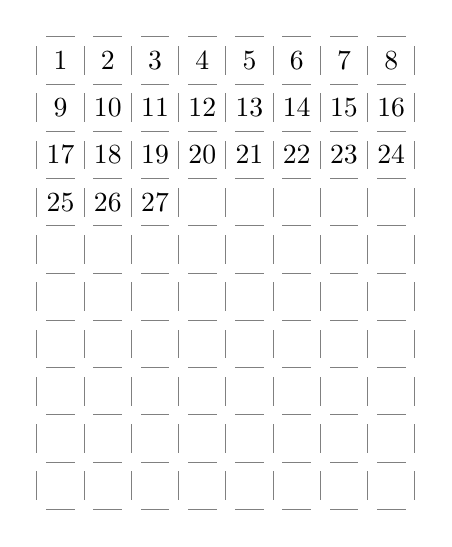
\begin{tikzpicture}[x=6mm,  y=6mm]
  \newcounter{num}
  \setcounter{num}{0}
  
  \draw[color=gray, step=6mm] (0,0) grid (8,10);
  \foreach \y in {9,8,...,0}{
    \foreach \x in {0,1,...,7}{
      \stepcounter{num}
      \ifnum \thenum<28
	\draw[xshift=3mm,yshift=3mm] (\x , \y ) node {\thenum};
      \fi
    }
  }
  
  \foreach \j in {10,9,8,...,0}
    \foreach \i in {0,1,...,8}
      \draw[] (\i , \j ) node[fill=white] {};
\end{tikzpicture}

  \boxA\quad~$x<5;x>3$\quad\boxB\quad~$3>x\ge~5$\quad\boxC\quad~$3\le x<5$\quad\boxD\quad~$3<x\le~5$
 \end{center}
  \end{esercizio}

\begin{esercizio}
 \label{ese:20.5}
Determina la scrittura corretta per il seguente grafico.
 \begin{center}
  % (c) 2012 Dimitrios Vrettos - d.vrettos@gmail.com

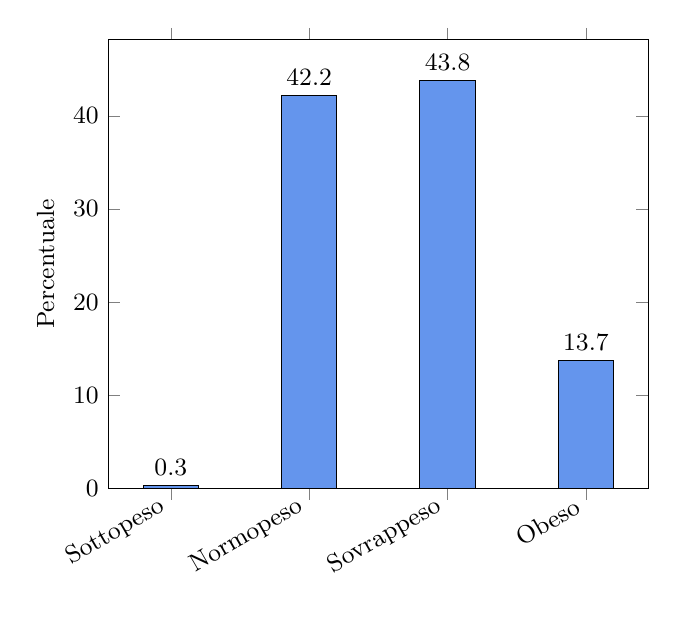
\begin{tikzpicture}[font=\small]
\begin{axis}[ymin=0,
ybar,
xtick=data,
ylabel=Percentuale,
x tick label style={rotate=30,anchor=east},
symbolic x coords={Sottopeso, Normopeso, Sovrappeso, Obeso},
bar width=20pt,enlarge x limits=0.15,nodes near coords,
nodes near coords align={vertical},
]
    \addplot[fill=CornflowerBlue,draw=black]
      coordinates{
	(Sottopeso, .3)
(Normopeso, 42.2)
(Sovrappeso, 43.8)
(Obeso,13.7)
      };
\end{axis}
\end{tikzpicture}


  \boxA\quad~$\insR^{-}-\{-1\}$\quad\boxB\quad~$-1\ge x\ge~0$\quad\boxC\quad~$-1\le x\le~0$\quad\boxD\quad~$0<x<-1$
 \end{center}
 \end{esercizio}

\begin{esercizio}
 \label{ese:20.6}
Determina la scrittura corretta per il seguente grafico.
 \begin{center}
  \input{./lbr/chap20/fig006_ret.pgf}

  \boxA\quad~$x>0$\quad\boxB\quad~$x>-\infty $\quad\boxC\quad~$x\le~0$\quad\boxD\quad~$0<x\le~0$
 \end{center}
  \end{esercizio}

\begin{esercizio}
 \label{ese:20.7}
Determina la scrittura corretta per il seguente grafico.
 \begin{center}
  % (c) 2012 Dimitrios Vrettos - d.vrettos@gmail.com
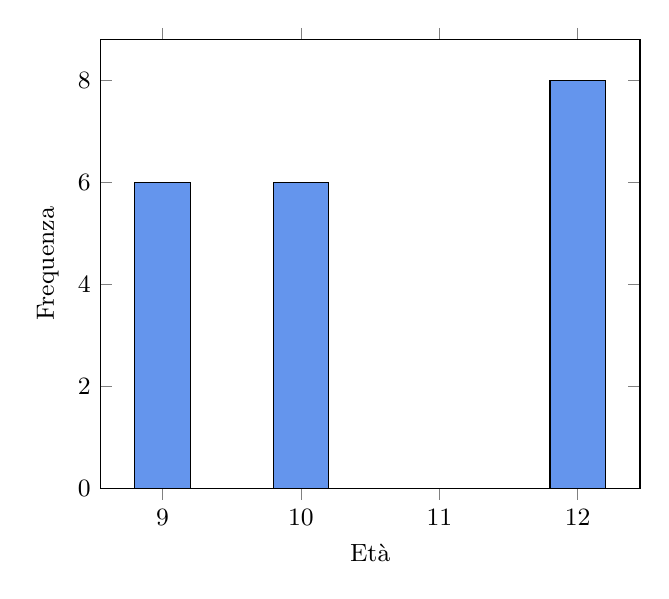
\begin{tikzpicture}[font=\small]

\begin{axis}[ymin=0,
ybar,
ylabel=Frequenza,
xlabel=Età,
bar width=20pt,
enlarge x limits=0.15,]

\addplot[fill=CornflowerBlue,draw=black]
      coordinates{
	(9, 6)
	(10,6)
	(12,8) };
\end{axis}
\end{tikzpicture}


  \boxA\quad~$x\ge~1;x<2$\quad\boxB\quad~$1\le x<2$\quad\boxC\quad~$x\le~1\text{ e }x>2$\quad\boxD\quad~$2\ge~1$
 \end{center}
  \end{esercizio}

\subsubsection*{20.2 - Disequazioni numeriche}
\begin{esercizio}
 \label{ese:20.8}
Completa la seguente tabella indicando con una crocetta il tipo di
disuguaglianza o disequazione:

 \begin{tabularx}{.9\textwidth}{Xccc}
 \toprule
 Proposizione&\multicolumn{2}{c}{Disuguaglianza}& Disequazione\\
  & Vera & Falsa & \\
 \midrule
 Il doppio di un numero reale è minore del suo triplo aumentato di~1: & & & \\
 La somma del quadrato di~4 con~3 è maggiore della somma del quadrato di~3 con~4: & & &\\
 Il quadrato della somma di~4 con~3 è minore o uguale a~49: & & & \\
 In~$\insZ:(5+8)-(2)^{4}>0$: & & & \\
 $-x^{2}>0$: & & & \\
 $(x+6)^{2}\cdot (1-9)\cdot (x+3-9)<0$: & & & \\
 \bottomrule
 \end{tabularx}
\end{esercizio}

\begin{esercizio}
 \label{ese:20.9}
 Rappresenta graficamente l'insieme delle soluzioni
delle seguenti disequazioni.
\begin{multicols}{3}
 \begin{enumeratea}
 \item $x-2>0$;
\item $x+5>0$;
\item $x-4>0$;
\item $x-5\ge~0$;
\item $x+3\le~0$;
\item $x>0$;
\item $x\ge~0$;
\item $-1\le x$;
\item $3>x$.
 \end{enumeratea}
\end{multicols}
\end{esercizio}

\begin{esercizio}[\Ast]
 \label{ese:20.10}
Trova l'Insieme Soluzione delle seguenti disequazioni.
\begin{multicols}{2}
 \begin{enumeratea}
 \item $3-x>x$;
\item $2x>3$;
\item $3x\le~4$;
\item $5x\ge -4$;
\item $x^{2}+x^{4}+10>0$;
\item $x^{2}+x^{4}+100<0$;
\item $-x+3>0$;
\item $-x-3\le~0$.
\end{enumeratea}
\end{multicols}
\end{esercizio}

\begin{esercizio}[\Ast]
 \label{ese:20.11}
Trova l'Insieme Soluzione delle seguenti disequazioni.
 \begin{multicols}{2}
 \begin{enumeratea}
 \item $3+2x\ge~3x+2$;
\item $5x-4\ge~6x-4$;
\item $-3x+2\ge -x-8$;
\item $4x+4\ge~2(2x+8)$;
\item $4x+4\ge~2(2x+1)$;
\item $4x+4\ge~2(2x+2)$;
\item $4x+4<2(2x+3)$;
\item $4x+4>2(2x+2)$.
\end{enumeratea}
\end{multicols}
\end{esercizio}

\begin{esercizio}[\Ast]
 \label{ese:20.12}
Trova l'Insieme Soluzione delle seguenti disequazioni.
 \begin{multicols}{2}
 \begin{enumeratea}
 \item $4x+4<2(2x+2)$;
\item $x^{2}+4>3$;
\item $x^{2}+3<-1$;
\item $-3x-8\ge~2$;
\item $-3x>0$;
\item $-3x\le~0$;
\item $-3x+5\ge~0$;
\item $-3x-8\ge~0$.
\end{enumeratea}
\end{multicols}
\end{esercizio}
\pagebreak
\begin{esercizio}[\Ast]
 \label{ese:20.13}
Trova l'Insieme Soluzione delle seguenti disequazioni.
 \begin{multicols}{2}
 \begin{enumeratea}
 \item $4x+4\ge~3\left(x+\frac{4}{3}\right)$;
\item $-{\dfrac{4}{3}}x\ge~1$;
\item $-{\dfrac{4}{3}}x\ge~0$;
\item $-{\dfrac{4}{3}}x\ge \dfrac{2}{3}$;
\item $-{\dfrac{2}{3}}x\le \dfrac{1}{9}$;
\item $-{\dfrac{2}{3}}x\le~9$;
\item $\dfrac{x+5}{2}>-{\dfrac{1}{5}}$;
\item $x^2+1\ge\dfrac{x^2+4x-1}{2}+3x$.
\end{enumeratea}
\end{multicols}
\end{esercizio}

\begin{esercizio}[\Ast]
 \label{ese:20.14}
Trova l'Insieme Soluzione delle seguenti disequazioni.
 \begin{multicols}{2}
 \begin{enumeratea}
 \item $x+\dfrac{1}{2}<\dfrac{(x+3)}{3}-1$;
\item $\dfrac{(x+5)}{3}+3+2\dfrac{(x-1)}{3}\le x+4$;
\item $(x+3)^{2}\ge (x-2)(x+2)$;
\item $\dfrac{3}{2}x+\dfrac{1}{4}<5\left(\dfrac{2}{3}x-\dfrac{1}{2}\right)$;
\item $1-(2x-4)^{2}>-x\cdot (4x+1)+2$;
\item $(x+1)^{2}\ge (x-1)^{2}$;
\item $\dfrac{3}{2}\cdot (x+1)-\dfrac{1}{3}\cdot (1-x)<x+2$;
\item $\dfrac{x+\np{0,25}}{2}<\np{1,75}+\np{0,25}x$.
\end{enumeratea}
\end{multicols}
\end{esercizio}

\begin{esercizio}[\Ast]
 \label{ese:20.15}
Trova l'Insieme Soluzione delle seguenti disequazioni.
 \begin{enumeratea}
 \item $\dfrac{1}{2}\left(3x-\dfrac{1}{3}\right)-\dfrac{1}{3}(1+x)(1-x)+3\left(\dfrac{1}{3}x-1\right)^{2}\ge~0$;
\item $3\dfrac{(x+1)}{2}-\dfrac{x+1}{3}-\dfrac{1}{9}>-5x+\dfrac{1}{2}$;
\item $\left(\dfrac{x}{2}-1\right)\left(1+\dfrac{x}{2}\right)+x-\dfrac{1}{2}>x\dfrac{(x-1)}{4}+\dfrac{5x-6}{4}$;
\item $\dfrac{1}{2}\left(x-\dfrac{1}{2}\right)+\dfrac{1}{3}\left(x+\dfrac{1}{3}\right)>\dfrac{x-\dfrac{1}{2}}{3}+\dfrac{x-\dfrac{1}{3}}{2}$.
\end{enumeratea}
\end{esercizio}
\begin{multicols}{2}
\begin{esercizio}[\Ast]
 \label{ese:20.16}
 Sommando un numero con il doppio del suo successivo si deve ottenere
un numero maggiore di~17. Quali numeri verificano questa
condizione?
\end{esercizio}

 \begin{esercizio}[\Ast]
 \label{ese:20.17}
 Sommando due numeri pari consecutivi si deve ottenere un numero che
non supera la metà del numero più grande. Quali valori può
assumere il primo numero pari?
 \end{esercizio}

 \begin{esercizio}[\Ast]
 \label{ese:20.18}
 Il noleggio di una automobile costa \officialeuro~$\np{55,00}$ al giorno, più
\officialeuro~$\np{0,085}$ per ogni chilometro percorso. Qual è il massimo di
chilometri da percorrere giornalmente, per spendere non più di \officialeuro~$\np{80,00}$ al giorno?
 \end{esercizio}

 \begin{esercizio}
 \label{ese:20.19}
 In una fabbrica, per produrre una certa merce, si ha
una spesa fissa settimanale di \officialeuro~$413$, ed un costo di produzione di \officialeuro~$\np{2,00}$ per ogni
kg di merce. Sapendo che la merce viene venduta a \officialeuro~$\np{4,00}$ al~kg, determinare la quantità minima da produrre
alla settimana perché l'impresa non sia in perdita.
 \end{esercizio}

 \begin{esercizio}[\Ast]
 \label{ese:20.20}
 Per telefonare in alcuni paesi esteri, una compagnia telefonica
propone due alternative di contratto:
\begin{enumeratea}
 \item \officialeuro~$\np{1,20}$ per il primo minuto di conversazione, \officialeuro~$\np{0,90}$ per ogni minuto successivo;
\item \officialeuro~$\np{1,00}$ per ogni minuto di conversazione.
\end{enumeratea}
Quanti minuti deve durare una telefonata perché convenga la seconda
alternativa?
 \end{esercizio}

\begin{esercizio}[\Ast]
 \label{ese:20.21}
 Il prezzo di un abbonamento mensile ferroviario è di \officialeuro~$\np{125,00}$.
 Sapendo che il prezzo di un singolo biglietto sulla stessa
tratta è di \officialeuro~$\np{9,50}$, trovare il numero minimo di viaggi per
cui l'abbonamento mensile risulta conveniente, e
rappresentare graficamente la soluzione.
 \end{esercizio}

 \begin{esercizio}
 \label{ese:20.22}
 Al circolo di tennis i soci pagano \officialeuro~$12$ a ora di gioco, mentre i non
soci pagano \officialeuro~$15$. Sapendo che la tessera annuale costa
\officialeuro~$150$, qual è il numero minimo di partite all'anno oltre il quale risulta conveniente
fare la tessera di socio?
 \end{esercizio}

 \begin{esercizio}[\Ast]
 \label{ese:20.23}
 \ In montagna l'abbonamento per due settimane allo
skipass costa \officialeuro~$220$ mentre il biglietto giornaliero costa
\officialeuro~$20$. Andando a sciare ogni giorno, dopo quanti giorni risulta coneniente
fare l'abbonamento?
 \end{esercizio}

 \begin{esercizio}[\Ast]
 \label{ese:20.24}
 Marco ha preso alle prime tre prove di matematica i seguenti voti: $5$;
$\np{5,5}$; $\np{4,5}$. Quanto deve prendere alla quarta e ultima prova per avere almeno~$6$
di media?
 \end{esercizio}

 \begin{esercizio}
 \label{ese:20.25}
 Per produrre un tipo di frullatore, un'azienda ha dei
costi fissi per \officialeuro~$\np{12000}$ a settimana e riesce a produrre~$850$
frullatori a settimana, ognuno dei quali ha un costo di produzione pari
a \officialeuro~$34$. L'azienda concorrente riesce a
vendere un frullatore analogo a \officialeuro~$79$. A quanto devono essere
venduti i frullatori in modo che l'azienda abbia un
utile e che il prezzo di vendita non sia superiore a quello del
prodotto concorrente?
 \end{esercizio}

 \begin{esercizio}[\Ast]
 \label{ese:20.26}
 Per il noleggio, una compagnia propone
un'auto di tipo citycar al costo di \officialeuro~$\np{0,20}$ per km percorso e una quota fissa giornaliera
di \officialeuro~$\np{15,00}$,
un'auto di tipo economy al costo di \officialeuro~$\np{0,15}$
per km e una quota fissa giornaliera di \officialeuro~$\np{20,00}$. Dovendo
noleggiare l'auto per~3 giorni, quanti km occorre fare
perché sia più conveniente l'auto di tipo economy?
 \end{esercizio}

 \begin{esercizio}
 \label{ese:20.27}
 Alle~9:00 di mattina sono in autostrada e devo raggiungere una città
che dista~$740\unit{km}$ entro le~17:00 poiché ho un appuntamento di lavoro.
Prevedendo una sosta di mezz'ora per mangiare un panino, a quale
velocità devo viaggiare per arrivare in orario?
 \end{esercizio}

 \begin{esercizio}[\Ast]
 \label{ese:20.28}
 Quanto deve essere lungo il lato di un triangolo equilatero il cui
perimetro deve superare di~$900\unit{cm}$ il perimetro di un triangolo
equilatero che ha il lato di~$10\unit{cm}$?
 \end{esercizio}

 \begin{esercizio}[\Ast]
 \label{ese:20.29}
 I lati di un triangolo sono tali che il secondo è doppio del primo e
il terzo è più lungo del secondo di~$3\unit{cm}$. Se il perimetro deve
essere compreso tra~$10\unit{cm}$ e~$20\unit{cm}$, tra quali valori può variare il lato
più piccolo?
 \end{esercizio}

 \begin{esercizio}[\Ast]
 \label{ese:20.30}
 In un triangolo isoscele l'angolo
alla base deve essere minore della metà dell'angolo
al vertice. Tra quali valori deve essere compresa la misura
dell'angolo alla base?
 \end{esercizio}

 \begin{esercizio}[\Ast]
 \label{ese:20.31}
 Un trapezio rettangolo ha l'altezza che è il triplo
della base minore, mentre la sua base maggiore è~5 volte quella minore.
Se il perimetro del trapezio non deve superare i~$100\unit{m}$, quali valori
può assumere la lunghezza dell'altezza del
trapezio?
 \end{esercizio}

 \begin{esercizio}[\Ast]
 \label{ese:20.32}
 Un rettangolo ha la lunghezza dei lati una doppia dell'altra.
Si sa che il perimetro non deve superare~$600\unit{m}$ e che
l'area non deve essere inferiore a~$200\unit{m^2}$. Tra quali
valori possono variare le dimensioni del rettangolo?
 \end{esercizio}
\end{multicols}
\pagebreak
 \subsubsection*{20.3 - Sistemi di disequazioni}

\begin{esercizio}
 \label{ese:20.33}
Sulla retta reale rappresenta l'insieme soluzione~$S_{1}$
dell'equazione:
\[\frac{1}{6}+\frac{1}{4}\cdot (5x+3)=2+\frac{2}{3}\cdot (x+1)\]
%\newpage
e l'insieme soluzione~$S_{2}$ della disequazione:
\[\frac{1}{2}-2\cdot\left(\frac{1-x}{4}\right)\ge~3-\frac{6-2x}{3}-\frac{x}{2}.\]

È vero che~$S_{1}\subset S_{2}$?
\end{esercizio}

\begin{esercizio}[\Ast]
 \label{ese:20.34}
 Determina i numeri reali che verificano il sistema:
 $\left\{%
  \begin{array}{l}
  x^{2}\le~0
  \\2-3x\ge~0
 \end{array}\right..$
 \end{esercizio}

\begin{esercizio}
 \label{ese:20.35}
 L'insieme soluzione del sistema:
$\left\{\begin{array}{l}
  (x+3)^{3}-(x+3)\cdot (9x-2)>x^{3}+27\\
  \dfrac{x+5}{3}+3+\dfrac{2\cdot (x-1)}{3}<x+1
 \end{array}\right.$ è:
\begin{multicols}{2}
\boxA\quad~$\left\{x\in \insR \mid x>3\right\}$

\boxB\quad~$\left\{x\in \insR \mid x>-3\right\}$

\boxC\quad~$\left\{x\in \insR \mid x<-3\right\}$

\boxD\quad~$\IS=\emptyset $

\boxE\quad~$\left\{x\in\insR \mid x<3\right\}$
\end{multicols}

\end{esercizio}

\begin{esercizio}
 \label{ese:20.36}
 Attribuire il valore di verità alle seguenti proposizioni:

\begin{enumeratea}
\item il quadrato di un numero reale è sempre positivo;
\item l'insieme complementare di~$A=\{x\in\insR\;|\;x>-8\}\text{ è }B=\{x\in\insR \mid x<-8\}$;
\item il monomio~$-6x^{3}y^{2}$ assume valore positivo per tutte le coppie dell'insieme~$\insR^{+}\times\insR^{+}$;
\item nell'insieme~$\insZ$ degli interi relativi il sistema~$\left\{\begin{array}{l}x+1>0\\8x<0\end{array}\right.$ non ha soluzione;
\item l'intervallo~$\left[-1\text{,~}\left.-{\dfrac{1}{2}}\right)\right.$ rappresenta l'$\IS$ del sistema~$\left\{\begin{array}{l}1+2x<0 \\\dfrac{x+3}{2}\le x+1\end{array}\right.$.
\end{enumeratea}
\end{esercizio}

\begin{esercizio}[\Ast]
 \label{ese:20.37}
 Risolvi i seguenti sistemi di disequazioni.
 \begin{multicols}{2}
 \begin{enumeratea}
 \item $\left\{\begin{array}{l}
	3-x>x\\
	2x>3
	\end{array}\right.;$
\item $\left\{\begin{array}{l}
	3x\le~4\\
	5x\ge -4
   \end{array}\right.;$
\item $\left\{\begin{array}{l}
	2x>3\\
	3x\le~4
	\end{array}\right.;$
\item $\left\{\begin{array}{l}
	3x-5<2\\
	x+7<-2x
   \end{array}\right..$
 \end{enumeratea}
\end{multicols}
\end{esercizio}

\begin{esercizio}[\Ast]
 \label{ese:20.38}
 Risolvi i seguenti sistemi di disequazioni.
 \begin{multicols}{2}
 \begin{enumeratea}
 \item $\left\{\begin{array}{l}
	3-x\ge x-3\\
	-x+3\ge~0
	\end{array}\right.;$
\item $\left\{\begin{array}{l}
	-x-3\le~3\\
	3+2x\ge~3x+2
   \end{array}\right.;$
\item $\left\{\begin{array}{l}
	2x-1>2x \\
	3x+3\le~3
	\end{array}\right.;$
\item $\left\{\begin{array}{l}
	2x+2<2x+3\\
	2(x+3)>2x+5
	\end{array}\right..$
\end{enumeratea}
\end{multicols}
\end{esercizio}

\begin{esercizio}[\Ast]
 \label{ese:20.39}
 Risolvi i seguenti sistemi di disequazioni.
 \begin{multicols}{2}
 \begin{enumeratea}
 \item $\left\{\begin{array}{l}
	-3x>0\\
	-3x+5\ge~0\\
	-3x\ge-2x
	\end{array}\right.;$
\item {\longarray $\left\{\begin{array}{l}
	-{\dfrac{4}{3}}x\ge\dfrac{2}{3}\\
	-{\dfrac{2}{3}}x\le\dfrac{1}{9}
	\end{array}\right.;$}
\item $\left\{\begin{array}{l}
	3+2x>3x+2 \\
	5x-4\le~6x-4\\
	-3x+2\ge -x-8
	\end{array}\right.;$
\item $\left\{\begin{array}{l}
	4x+4\ge~3\cdot\left(x+\dfrac{4}{3}\right)\\
	4x+4\ge~2\cdot (2x+2)
	\end{array}\right..$
\end{enumeratea}
\end{multicols}
\end{esercizio}

\begin{esercizio}[\Ast]
 \label{ese:20.40}
 Risolvi i seguenti sistemi di disequazioni.
 \begin{multicols}{2}
 \begin{enumeratea}
 \item $\left\{\begin{array}{l}
	3(x-1)<2(x+1)\\
	x-\dfrac{1}{2}+\dfrac{x+1}{2}>0
	\end{array}\right.;$
\item {\longarray $\left\{\begin{array}{l}
	16(x+1)-2+(x-3)^{2}\le(x+5)^{2}\\
	\dfrac{x+5}{3}+3+2\cdot\dfrac{x-1}{3}\le x+4
	\end{array}\right.;$}
\item $\left\{\begin{array}{l}
	x+\dfrac{1}{2}<\dfrac{1}{3}(x+3)-1\\
	(x+3)^{2}\ge (x-2)(x+2)
	\end{array}\right.;$
\item {\longarray $\left\{\begin{array}{l}
	\dfrac{2x+3}{3}>x-1\\
	\dfrac{x-4}{5}<\dfrac{2x+1}{3}
	\end{array}\right..$}
\end{enumeratea}
\end{multicols}
\end{esercizio}

\begin{esercizio}[\Ast]
 \label{ese:20.41}
 Risolvi i seguenti sistemi di disequazioni.

 \begin{enumeratea}
 \item {\longarray $\left\{\begin{array}{l}
	2\left(x-\dfrac{1}{3}\right)+x>3x-2\\
	\dfrac{x}{3}-\dfrac{1}{2}\ge \dfrac{x}{4}-\dfrac{x}{6}
   \end{array}\right.;$}
\item $\left\{\begin{array}{l}
    \dfrac{3}{2}x+\dfrac{1}{4}<5\cdot\left(\dfrac{2}{3}x-\dfrac{1}{2}\right)\\
    x^2-2x+1\ge~0
   \end{array}\right.;$
\item {\longarray $\left\{\begin{array}{l}
	3\left(x-\dfrac{4}{3}\right)+\dfrac{2-x}{3}+x-\dfrac{x-1}{3}>0\\
	\left[1-\dfrac{1}{6}(2x+1)\right]+\left(x-\dfrac{1}{2}\right)^{2}<(x+1)^{2}+\dfrac{1}{3}(1+2x)
   \end{array}\right.;$}
\item {\longarray $\left\{\begin{array}{l}
	\left(x-\dfrac{1}{2}\right)\left(x+\dfrac{1}{2}\right)>\left(x-\dfrac{1}{2}\right)^{2}\\
	2\left(x-\dfrac{1}{2}\right)\left(x+\dfrac{1}{2}\right)<\left(x-\dfrac{1}{2}\right)^{2}+\left(x+\dfrac{1}{2}\right)^{2}
   \end{array}\right..$}
 \end{enumeratea}
\end{esercizio}

\subsubsection*{20.4 - Disequazioni polinomiali di grado superiore al primo}
\begin{esercizio}
 \label{ese:20.42}
 Mediante il metodo~1 del problema~\ref{pro:20.1} (a pagina \pageref{pro:20.1}) risolvi le seguenti disequazioni.

\begin{enumeratea}
\item $(x+3)\cdot \left(\frac{1}{5}x+\frac{3}{2}\right)<0$ e~$\left(-{\frac{6}{11}}+2x\right)\cdot\left(-x+\frac{9}{2}\right)$;
\item $\left(x+\frac{3}{2}\right)\cdot \left(5x+\frac{1}{5}\right)<0$ e~$\left(-{\frac{1}{10}}x+2\right)\cdot \left(-3x+9\right)\ge~0$.
\end{enumeratea}

\end{esercizio}

\begin{esercizio}
 \label{ese:20.43}
 Il metodo~1 del problema~\ref{pro:20.1} (a pagina \pageref{pro:20.1}) si complica se il prodotto ha
più di due fattori. Prova infatti ad applicarlo alla seguente
disequazione:
$(x-3)\cdot (2x-9)\cdot (4-5x)>0.$
\end{esercizio}
\pagebreak

\begin{esercizio}[\Ast]
 \label{ese:20.44}
Trova l'Insieme Soluzione delle seguenti disequazioni.
\begin{multicols}{2}
 \begin{enumeratea}
 \item $(x+2)(3-x)\le~0$;
\item $x(x-2)>0$;
\item $(3x+2)(2-3x)<0$;
\item $-3x(2-x)(3-x)\ge~0$.
\end{enumeratea}
\end{multicols}
\end{esercizio}

\begin{esercizio}[\Ast]
 \label{ese:20.45}
Trova l'Insieme Soluzione delle seguenti disequazioni.
\begin{multicols}{2}
 \begin{enumeratea}
 \item $(x+1)(1-x)\left(\frac{1}{2}x-2\right)\ge~0$;
\item $(x-1)(x-2)(x-3)(x-4)<0$;
\item $x^{2}-16\le~0$;
\item $4x^{2}-2x<0$.
\end{enumeratea}
\end{multicols}
\end{esercizio}

\begin{esercizio}[\Ast]
 \label{ese:20.46}
Trova l'Insieme Soluzione delle seguenti disequazioni.
\begin{multicols}{2}
 \begin{enumeratea}
 \item $x^{4}-81\ge~0$;
\item $x^{2}+17x+16\le~0$;
\item $16-x^{4}\le~0$;
\item $x^{2}+2x+1<0$.
\end{enumeratea}
\end{multicols}
\end{esercizio}

\begin{esercizio}[\Ast]
 \label{ese:20.47}
Trova l'Insieme Soluzione delle seguenti disequazioni.
\begin{multicols}{2}
 \begin{enumeratea}
 \item $x^{2}+6x+9\ge~0$;
\item $x^{2}-5x+6<0$;
\item $x^{2}+3x-4\le~0$;
\item $x^{3}>x^{2}$.
\end{enumeratea}
\end{multicols}
\end{esercizio}

\begin{esercizio}[\Ast]
 \label{ese:20.48}
Trova l'Insieme Soluzione delle seguenti disequazioni.
\begin{multicols}{2}
 \begin{enumeratea}
 \item $x^{2}(2x^{2}-x)-(2x^{2}-x)<0$;
\item $x^{2}-2x+1+x(x^{2}-2x+1)<0$;
\item $x^{3}-2x^{2}-x+2\ge~0$;
\item $x^{4}+4x^{3}+3x^{2}>0$.
\end{enumeratea}
\end{multicols}
\end{esercizio}

\begin{esercizio}[\Ast]
 \label{ese:20.49}
Trova l'Insieme Soluzione delle seguenti disequazioni.
\begin{multicols}{2}
 \begin{enumeratea}
 \item $(6x^{2}-24x)(x^{2}-6x+9)<0$;
\item $(x^{3}-8)(x+2)<(2-x)(x^{3}+8)$;
\item $(2a+1)(a^{4}-2a^{2}+1)<0$;
\item $x^{3}-6x^{2}+11>1-3x$;
\item $x^{6}-x^{2}+x^{5}-6x^{4}-x+6<0$.
\end{enumeratea}
\end{multicols}
\end{esercizio}

\begin{esercizio}[\Ast]
 \label{ese:20.50}
 Determina i valori che attribuiti alla variabile~$y$ rendono positivi
entrambi i polinomi
seguenti:~$p_{1}=y^{4}-13y^{2}+36;\quad p_{2}=y^{3}-y^{2}-4y+4.$
\end{esercizio}

\begin{esercizio}[\Ast]
 \label{ese:20.51}
 Determina i valori di~$a$ che rendono~$p=a^{2}+1$ minore di~5.
\end{esercizio}

\begin{esercizio}[\Ast]
 \label{ese:20.52}
 Determina~$\IS$ dei seguenti sistemi di disequazioni.
 \begin{multicols}{3}
 \begin{enumeratea}
 \item $\left\{\begin{array}{l}
		x^{2}-9\ge~0\\
		x^{2}-7x+10<0
	   \end{array}\right.;$
\item $\left\{\begin{array}{l}
		x^{2}+3x-18\ge~0\\
		12x^{2}+12x+3>0
	   \end{array}\right.;$
\item $\left\{\begin{array}{l}
		16x^{4}-1<0 \\
		16x^{3}+8x^{2}\ge~0 \end{array}\right.. $
 \end{enumeratea}
 \end{multicols}
\end{esercizio}

\begin{esercizio}[\Ast]
 \label{ese:20.53}
 Determina~$\IS$ dei seguenti sistemi di disequazioni.
 \begin{multicols}{2}
 \begin{enumeratea}
 \item $\left\{\begin{array}{l}
		49a^{2}-1\ge~0\\
		9a^{2}<1\\
		1-a>0
	   \end{array}\right.;$

\item $\left\{\begin{array}{l}
	  2x^{2}-13x+6<0\\
	  (2x^{2}-5x-3)(1-3x)>0\\
	  x^{2}+7>1
	   \end{array}\right..$
 \end{enumeratea}
 \end{multicols}
\end{esercizio}

\begin{esercizio}
\label{ese:20.54}
Studia il segno della frazione
\[f=\dfrac{x^{3}+11x^{2}+35x+25}{x^{2}-25}.\]
\emph{Traccia di svolgimento}. Scomponi in fattori numeratore e denominatore, otterrai
\[ f=\frac{(x+5)^{2}(x+1)}{(x+5)(x-5)}.\]
Poni le~$\CE$ e semplifica la frazione: \dotfill

Studia separatamente il segno di tutti i fattori che vi compaiono. Verifica che la tabella dei segni sia:
\begin{center}
% (c) 2012 Dimitrios Vrettos - d.vrettos@gmail.com
\begin{tikzpicture}[font=\small,x=10mm, y=10mm]

\draw[->] (0,0) -- (8,0) node [below right] () {$r$};

\foreach \x in {1.5,3.5,6.5}{
\draw(\x,3pt)--(\x,-3pt);
\begin{scope}[dotted]
\draw (\x,0) -- (\x,-2);
\draw (0,-.5) -- (1.5,-.5);
\draw (0,-1) -- (3.5,-1);
\draw (0,-1.5) -- (6.5,-1.5);
\end{scope}}


\node[above] at (1.5,0) {$-5$};
\node[above]  at (3.5,0) {$-1$};
\node[above]  at (6.5,0) {$5$};

\begin{scope}[blue,thick]
\draw (1.5,-.5) -- (8,-.5);
\draw (3.5,-1) -- (8,-1);
\draw (6.5,-1.5) -- (8,-1.5);

\draw[fill=white] (1.5,-.5)circle (1.5pt);
\draw[fill=blue] (3.5,-1)circle (1.5pt);
\draw[fill=white] (6.5,-1.5)circle (1.5pt);
\end{scope}

\foreach \x in {-1.5}{
\node (n1) at (\x,-.25) {segno di $n_1$:};
\node(n2)  at (\x,-.75) {segno di $n_2$:};
\node   at (\x,-1.25) {segno di $D$:};
\node (d3) at (\x,-1.75) {segno di $f$:};
}

 \draw[decorate, decoration={brace, mirror}]  let \p1=(n1.north west), \p2=(n2.south west) in(\p1 ) -- (\p2) node[midway, left=2pt] {$N:$};

\foreach \z in {2.5,5,7.25}
\node  at (\z,-.25) {$+$};

 \foreach \zi in {.75,2.5}
 \node  at (\zi,-.75) {$-$};

\foreach \zii in {5,7.25}
 \node  at (\zii,-.75) {$+$};

 \foreach \ziii in {.75,2.5,5}
\node  at (\ziii,-1.25) {$-$};

\node  at (.75,-.25) {$-$};
\node  at (7.25,-1.25) {$+$};

\begin{scope}[red]
\foreach \y in {-1.75}{
\foreach \ziv in {.75,5}
	\node at (\ziv,\y) {$-$};
\foreach \zv in {2.5,7.25}
\node at (\zv,\y) {$+$};
}
\end{scope}
\end{tikzpicture}
\end{center}
La frazione assegnata, con la~$\CE: x\neq -5\text{ e }x\neq~5$, si annulla se~$x=-1$;
è positiva nell'insieme~$A^{+}=\left\{x\in \insR | -5<x<-1\vee x>5\right\}$ ed è negativa in
$A^{-}=\left\{x\in\insR | x<-5\vee -1<x<5\right\}$.
\end{esercizio}

\begin{esercizio}[\Ast]
\label{ese:20.55}
Determina~$\IS$ delle seguenti disequazioni fratte.
\begin{multicols}{2}
\begin{enumeratea}
\spazielenx
\item $\dfrac{x-2}{3x-9}>0$;
\item $\dfrac{3x+12}{(x-4)(6-3x)}\geqslant~0$;
\item $\dfrac{x+2}{x-1}<2$;
\item $\dfrac{4-3x}{6-5x}\geqslant -3$.
\end{enumeratea}
\end{multicols}
\end{esercizio}

\begin{esercizio}[\Ast]
\label{ese:20.56}
Determina~$\IS$ delle seguenti disequazioni fratte.
\begin{multicols}{2}
\begin{enumeratea}
\spazielenx
 \item $\dfrac{x+8}{x-2}\ge~0$;
\item $\dfrac{3x+4}{x^{2}+1}\ge~2$;
\item $\dfrac{4}{x+4}+\dfrac{2}{x-3}\leqslant~0$;
\item $\dfrac{7}{x+3}-\dfrac{6}{x+9}\geqslant~0$.
\end{enumeratea}
\end{multicols}
\end{esercizio}

\begin{esercizio}[\Ast]
\label{ese:20.57}
Determina~$\IS$ delle seguenti disequazioni fratte.
\begin{multicols}{2}
\begin{enumeratea}
\spazielenx
 \item $\dfrac{3}{2-x}\leqslant \dfrac{1}{x-4}$;
\item $\dfrac{2}{4x-16}<\dfrac{2-6x}{x^{2}-8x+16}$;
\item $\dfrac{x-3}{x^{2}-4x+4}-1<\dfrac{3x-3}{6-3x}$;
\item $\dfrac{2}{x-2}>\dfrac{2x-2}{(x-2)(x+3)}$.
\end{enumeratea}
\end{multicols}
\end{esercizio}

\begin{esercizio}[\Ast]
\label{ese:20.58}
Determina~$\IS$ delle seguenti disequazioni fratte.
\begin{multicols}{2}
\begin{enumeratea}
\spazielenx
 \item $\dfrac{5}{2x+6}\geqslant \dfrac{5x+4}{x^{2}+6x+9}$;
\item $\dfrac{x}{x+1}-\dfrac{1}{x^{3}+1}\le~0$;
\item $\dfrac{(x+3)(10x-5)}{x-2}<0$;
\item $\dfrac{4-3x}{x-2}<\dfrac{3x+1}{x-2}$.
\end{enumeratea}
\end{multicols}
\end{esercizio}

\begin{esercizio}[\Ast]
\label{ese:20.59}
Determina~$\IS$ delle seguenti disequazioni fratte.
\begin{multicols}{2}
\begin{enumeratea}
\spazielenx
 \item $\dfrac{5x-4}{3x-12}\ge \dfrac{x-4}{4-x}$;
\item $\dfrac{2-x}{5x-15}\le \dfrac{5x-1}{2x-6}$;
\item $\dfrac{(3x-12)(6-x)}{(24-8x)(36-18x)}\leqslant~0$;
\item $\dfrac{(x-2)(5-2x)}{(5x-15)(24-6x)}\geqslant~0$.
\end{enumeratea}
\end{multicols}
\end{esercizio}
%\newpage
\begin{esercizio}[\Ast]
\label{ese:20.60}
Determina~$\IS$ delle seguenti disequazioni fratte.
\begin{multicols}{2}
\begin{enumeratea}
\spazielenx
\item $\dfrac{(x-2)(x+4)(x+1)}{(x-1)(3x-9)(10-2x)}\leqslant~0$;
\item $\dfrac{(5-x)(3x+6)(x+3)}{(4-2x)(x-6)x}\leqslant~0$;
\item $\dfrac{(x-5)(3x-6)(x-3)}{(4-2x)(x+6)x}\leqslant~0$;
\item $\dfrac{(x-3)(x+2)(15+5x)}{x^{2}-5x+4}\geqslant~0$.
\end{enumeratea}
\end{multicols}
\end{esercizio}

\begin{esercizio}[\Ast]
\label{ese:20.61}
Determina~$\IS$ delle seguenti disequazioni fratte.
\begin{multicols}{2}
\begin{enumeratea}
\spazielenx
\item $\dfrac{\left(x-4\right)^{2}(x+3)}{x^{2}+5x+6}\geqslant~0$;
\item $\dfrac{x}{1-x^{2}}>\dfrac{1}{2x+2}-\dfrac{2}{4x-4}$;
\item $\dfrac{3-x}{x-2}<\dfrac{x-1}{x+3}+\dfrac{2}{x^{2}+x-6}$;
\item $\dfrac{2}{x+2}-\dfrac{1}{x+1}\ge \dfrac{3}{2x+2}$.
\end{enumeratea}
\end{multicols}
\end{esercizio}

\begin{esercizio}[\Ast]
\label{ese:20.62}
Determina~$\IS$ delle seguenti disequazioni fratte.
\begin{multicols}{2}
\begin{enumeratea}
\spazielenx
 \item $\dfrac{3}{2x-1}\le \dfrac{2x^{2}}{2x^{2}-x}-\dfrac{x+1}{x}$;
\item $\dfrac{2x^{2}}{2x^{2}-x}>1$;
\item $\dfrac{2x}{2x-1}+\dfrac{x+2}{2x+1}>\dfrac{3}{2}$;
\item $\dfrac{x^{2}-5x+6}{x^{2}-7x+12}\le~1$.
\end{enumeratea}
\end{multicols}
\end{esercizio}

\begin{esercizio}[\Ast]
\label{ese:20.63}
Determina~$\IS$ delle seguenti disequazioni fratte.
\begin{multicols}{2}
\begin{enumeratea}
\spazielenx
 \item $\dfrac{\dfrac{2}{x+1}}{x^{2}-1}<0$;
\item $\dfrac{x}{x+1}-\dfrac{4-x}{x+2}\ge \dfrac{2x+1}{x^{2}+3x+2}$;
\item $\dfrac{3}{2x^{2}-4x-6}-\dfrac{x-2}{3x+3}<\dfrac{x-1}{2x-6}$;
\item $\dfrac{1}{2-2x}\cdot \left(\dfrac{x(x-2)}{x-1}-\dfrac{3}{3-3x}\right)>-1$.
\end{enumeratea}
\end{multicols}
\end{esercizio}

\begin{esercizio}[\Ast]
\label{ese:20.64}
Determina~$\IS$ delle seguenti disequazioni fratte.

\begin{enumeratea}
 \item $-{\dfrac{2}{27-3x^{2}}}-\dfrac{x+1}{2x-6}+\dfrac{3-2x}{6x-18}<-{\dfrac{3}{x^{2}-9}}+4\dfrac{x-3}{18-2x^{2}}$;
\item $\dfrac{2}{x^{2}-3x+2}-\dfrac{x}{x-2}<\dfrac{x-1}{x-1}-\dfrac{1}{3x-x^{2}-2}+\dfrac{2-x}{4x-4}$;
\item $\dfrac{(x-2)(x+4)(x^{2}+5x+6)}{(x^{2}-9)(-4-7x^{2})(x^{2}-6x+8)(x^{2}+4)}<0$.
\end{enumeratea}
\end{esercizio}
\pagebreak
\begin{esercizio}
\label{ese:20.65}
Dopo aver ridotto ai minimi termini la frazione
$f=\dfrac{3x^{4}-2x^{3}+3x^{2}-2x}{6x^{2}-x-7}$, completa

 \begin{enumeratea}
 \item $f>0$ per~$x<-1$ oppure \dotfill
 \item $f=0$ per \dotfill
 \item $f<0$ per \dotfill
 \end{enumeratea}
\end{esercizio}

\begin{esercizio}
\label{ese:20.66}
Determina il segno delle frazioni, dopo averle ridotte ai minimi termini.
\[f_{1}=\dfrac{1-a^{2}}{2+3a};\quad f_{2}=\dfrac{a^{3}-5a^{2}-3+7a}{9-6a+a^{2}};\quad f_{3}=\dfrac{11m-m^{2}+26a}{(39-3m)(m^{2}+4m+4)}.\]
\end{esercizio}

\begin{esercizio}[\Ast]
\label{ese:20.67}
Determina~$\IS$ delle seguenti disequazioni fratte.

\begin{enumeratea}{\longarray
 \item $\left\{\begin{array}{l}
		\dfrac{2-x}{3x^{2}+x}\ge~0\\
		x^{2}-x-6\ge~0\\
		x^{2}-4\le~0
	\end{array}\right.;$
\item $\left\{\begin{array}{l}
        \dfrac{x^{2}-4x+4}{9-x^{2}>0}\\
        x^{2}-3x\le~0
       \end{array}\right.;$
\item $\left\{\begin{array}{l}
	   \dfrac{1}{x-2}+\dfrac{3}{x+2}<0\\
	   \dfrac{2-x}{5x-15}\le\dfrac{5x-1}{2x-6}
	   \end{array}\right.;$
\item $\left\{\begin{array}{l}
	   \dfrac{4}{8-4x}-\dfrac{6}{2x-4}<0\\
	   \dfrac{x}{x-2}-\dfrac{6}{x^{3}-8}>1
	   \end{array}\right.;$
\item $\left\{\begin{array}{l}
	   \left(1+\dfrac{2}{x-2}\right)\left(1-\dfrac{2}{x-2}\right)<\dfrac{x-4}{2-x}\\
	   \left(\dfrac{2-x}{x^{2}-6x+9}+\dfrac{2+x}{x^{2}-9}\right)\cdot{\dfrac{x^{3}-27}{2x}}>0
	   \end{array}\right..$}
\end{enumeratea}

\end{esercizio}

\begin{esercizio}[\Ast]
\label{ese:20.68}
Determina~$\IS$ delle seguenti disequazioni fratte.
\begin{multicols}{2}
\begin{enumeratea}{\longarray
 \item $\left\{\begin{array}{l}
		\left(1-\dfrac{1}{x}\right)+3\left(\dfrac{2}{x}+1\right)>\dfrac{13}{2}\\
		\dfrac{7+x}{2x}>\dfrac{2-x}{1-2x}
   \end{array}\right.;$
\item $\left\{\begin{array}{l}
		\dfrac{x^{2}-2x-3}{2x^{2}-x-1}\ge~0\\
		\dfrac{4x-1-3x^{2}}{x^{2}-4}\le~0
	\end{array}\right.;$
\item $\left\{\begin{array}{l}
		x^{2}-3x+2\le0\\
		\dfrac{6}{2+x}-\dfrac{x+2}{x-2}>\dfrac{x^{2}}{4-x^{2}}
	\end{array}\right.;$
\item $\left\{\begin{array}{l}
		x^{2}+1\le -2x\\
		3x-1<2\left(x-\dfrac{1}{2}\right)
		\end{array}\right..$}
\end{enumeratea}
\end{multicols}
\end{esercizio}

\begin{esercizio}
\label{ese:20.69}
Motiva la verità o la falsità delle seguenti
proposizioni riferite alle frazioni.
\begin{multicols}{3}
\noindent\[f_{1}=\frac{a^{3}-81a}{81-a^{2}}\text{,}\]
\[f_{2}=\frac{7a^{2}+7}{3+3a^{4}+6a^{2}}\text{,}\]
\[f_{3}=\frac{20a-50a^{2}-2}{4a-20a^{2}}\text{,}\]
\[f_{4}=\frac{a^{4}}{2a^{4}+a^{2}}\text{,}\]
\[f_{5}=\frac{1-4a^{2}}{2-8a+8a^{2}}\text{,}\]
\[f_{6}=\frac{2a^{2}+a^{3}+a}{2a^{2}-a^{3}-a}.\]
\end{multicols}
\begin{enumeratea}
\TabPositions{11cm}
\item $f_{1}$ per qualunque valore positivo della variabile è negativa \tab\boxV\quad\boxF
\item $f_{2}$ è definita per qualunque valore attribuito alla variabile \tab\boxV\quad\boxF
\item $f_{3}$ è positiva nell'insieme~$\IS=\left\{a\in \insR\;|\;a<0\vee a>\frac{1}{5}\right\}$ \tab\boxV\quad\boxF
\item $f_{4}$ è positiva per qualunque valore reale attribuito alla variabile \tab\boxV\quad\boxF
\item $f_{5}$ non si annulla nell'intervallo~$\left[-\frac{1}{2}\text{,~}\frac{1}{2}\right)$ \tab\boxV\quad\boxF
\item $f_{6}$ è negativa per qualunque valore dell'insieme~$K=\insR-\{-1\text{,~}0\text{,~}1\}$ \tab\boxV\quad\boxF
\end{enumeratea}
\end{esercizio}

\subsection{Risposte}
\paragraph{20.10.} a)~$x<\frac{3}{2}$,\quad b)~$x>\frac{3}{2}$,\quad
c)~$x\le \frac{4}{3}$,\quad d)~$x\ge -{\frac{4}{5}}$,\quad
e)~$\insR$,\quad f)~$\emptyset $,\quad
g)~$x<3$,\quad \protect\\ h)~$x\ge -3$.

\paragraph{20.11.} a)~$x\le~1$,\quad b)~$x\le~0$,\quad
c)~$x\le~5$,\quad d)~$\emptyset $,\quad
e)~$\insR$,\quad f)~$\insR$,\quad
g)~$\insR $,\quad h)~$\emptyset $.

\paragraph{20.12.} a)~$\emptyset $,\quad b)~$\insR$,\quad
c)~$\emptyset $,\quad d)~$x\le -{\frac{10}{3}}$,\quad
e)~$x<0$,\quad f)~$x\ge~0$,\quad
g)~$x\le \frac{5}{3}$,\quad h)~$x\le -{\frac{8}{3}}$.

\paragraph{20.13.} a)~$x\ge~0$,\quad b)~$x\le -{\frac{3}{4}}$,\quad
c)~$x\le~0$,\quad d)~$x\le -{\frac{1}{2}}$,\quad
e)~$x\ge -{\frac{1}{6}}$,\quad f)~$x\ge -{\frac{27}{2}}$,\quad
\protect\\g)~$x>-{\frac{27}{5}}$,\quad h)~$\insR$.

\paragraph{20.14.} a)~$x<-{\frac{3}{4}}$,\quad b)~$\insR$,\quad
c)~$x\ge -{\frac{13}{6}}$,\quad d)~$x>\frac{3}{2}$,\quad
e)~$x>1$,\quad f)~$x\ge~0$,\quad\protect\\
g)~$\{x\in\insR/x<1\}=(-\infty,1)$,\quad h)~$x<\frac{13}{2}$.

\paragraph{20.15.} a)~$\insR$,\quad b)~$x>-{\frac{10}{111}}$,\quad
c)~$\emptyset $,\quad d)~$\insR$.

\begin{multicols}{2}
\paragraph{20.16.} $x>5$.

\paragraph{20.17.} $x\le -2/3$.

\paragraph{20.18.} Massimo~$294\unit{km}$.

\paragraph{20.20.} Meno di~3 minuti.

\paragraph{20.21.} 14

\paragraph{20.23.} $x>11$.

\paragraph{20.24.} Almeno~9.

\paragraph{20.26.} Più di~$300\unit{km}$.

\paragraph{20.28.} $x>310\unit{cm}$.

\paragraph{20.29.} $\frac{7}{5}\unit{cm}<x<\frac{17}{5}\unit{cm}$.

\paragraph{20.30.} $0^{\circ}<\alpha<45^{\circ}$.

\paragraph{20.31.} $h\le \frac{150}{7}m$.
\end{multicols}

\paragraph{20.32.} Il lato minore tra~$10\unit{m}$ e~$100\unit{m}$, il lato maggiore tra~$20\unit{m}$ e~$200\unit{m}$.

\paragraph{20.34.} $x = 0$.

\paragraph{20.37.} a)~$\emptyset $,\quad b)~$-{\frac{4}{5}}\le x\le\frac{4}{3}$,\quad c)~$\emptyset $,\quad
\protect\\ d)~$x<-{\frac{7}{3}}$.

\paragraph{20.38.} a)~$x\le~3$,\quad b)~$-6\le x\le~1$,\quad c)~$\emptyset $,\quad d)~$\insR$.

\paragraph{20.39.} a)~$x<0$,\quad b)~$\emptyset $,\quad c)~$0\le x<1$,\quad d)~$x\ge~0$.

\paragraph{20.40.} a)~$0<x<5$,\quad b)~$\insR$,\quad
\quad c)~$-{\frac{13}{6}}\le x<-{\frac{3}{4}}$,\quad d)~$-{\frac{17}{7}}<x<6$.

\paragraph{20.41.} a)~$x\ge~2$,\quad b)~$x>\frac{3}{2}$,\quad c)~$x>\frac{9}{10}$,\quad d)~$x>\frac{1}{2}$.

\paragraph{20.44.} a)~$x\le -2\vee x\ge~3$,\quad b)~$x<0\vee x>2$,\quad
c)~$x<-{\frac{2}{3}}\vee x>\frac{2}{3}$,\quad d)~$x\ge~0\vee~2\le x\le~3$.

\paragraph{20.45.} a)~$x\le -1\vee~1\le x\le4$,\quad b)~$1<x<2\vee~3<x<4$,\quad
c)~$-4\le x\le~4$,\quad d)~$0<x<\frac{1}{2}$.

\paragraph{20.46.} a)~$x\le -3\vee x\ge~3$,\quad b)~$-16\le x\le -1$,\quad
c)~$x\le -2\vee x\ge~2$,\quad d)~$\emptyset $.

\paragraph{20.47.} a)~$\insR$,\quad b)~$2<x<3$,\quad
c)~$-4\le x\le~1$,\quad d)~$x>1$.

\paragraph{20.48.} a)~$-1<x<0\vee \frac{1}{2}<x<1$,\quad b)~$x<-1$,\quad
c)~$-1\le x\le~1\vee x\ge~2$,\quad \protect\\ d)~$x<-3\vee x>-1\wedge x\neq~0$.

\paragraph{20.49.} a)~$0<x<4\wedge x\neq~3$,\quad b)~$-2<x<2$,\quad
c)~$a<-{\frac{1}{2}}\wedge a\neq -1$,\quad d)~$-1<x<2\vee x>5$,\quad e)~$-3<x<-1\vee~1<x<2$.

\paragraph{20.50.} $-2<y<1\vee y>3$.

\paragraph{20.51.} $-2<a<2$.

\paragraph{20.52.} a)~$3\le x<5$,\quad b)~$x\le -6\vee x\ge~3$,\quad
c)~$-{\frac{1}{2}}<x<\frac{1}{2}$.

\paragraph{20.53.} a)~$-{\frac{1}{3}}<a\le -{\frac{1}{7}}\vee \frac{1}{7}\le a<\frac{1}{3}$,\quad
b)~$\frac{1}{2}<x<3$.

\paragraph{20.55.} a)~$x<2\vee x>3$,\quad b)~$x\le -4\vee~2<x<4$,\quad
c)~$x<1\vee x>4$,\quad d)~$x<\frac{6}{5}\vee x\ge\frac{11}{9}$.

\paragraph{20.56.} a)~$x\le -8\vee x>2$,\quad b)~$-{\frac{1}{2}}\le x\le~2$,\quad
c)~$x<-4\vee\frac{2}{3}\le x<3$,\quad \protect\\ d)~$-45\le x<-9\vee x>-3$.

\paragraph{20.57.} a)~$2<x\le \frac{7}{2}\vee x>4$,\quad
b)~$x<\frac{8}{13}$,\quad
c)~$x<2\vee~2<x<\frac{5}{2}$,\quad d)~$x<-3\vee x>2$.

\paragraph{20.58.} a)~$x\le \frac{7}{5}\wedge x\neq-3$,\quad
b)~$-1<x\le~1$,\quad
\protect\\ c)~$x<-3\vee\frac{1}{2}<x<2$,\quad d)~$x<\frac{1}{2}\vee x>2$.

\paragraph{20.59.} a)~$x\le~2\vee x>4$,\quad b)~$x\le \frac{1}{3}\vee x>3$,\quad
c)~$x<2\vee~3<x\le~4\vee x\ge~6$,\quad \protect\\ d)~$x\le~2\vee \frac{5}{2}\le x<3\vee x>4$.

\paragraph{20.60.} a)~$x\le -4\vee -1\le x<1\vee~2\le x<3\vee x>5$,\quad
\protect\\ b)~$-3\le x\le -2\vee~0<x<2\vee~5\le x<6$,\quad
c)~$x<-6\vee~0<x\le3\vee x\ge~5\text{ con }x\neq~2$,\quad d)~$-3\le x\le -2\vee~1<x\le~3\vee x>4$.

\paragraph{20.61.} a)~$x>-2$,\quad b)~$x<-1$,\quad
c)~$x<-3\vee -1<x<2\vee x>\frac{5}{2}$,\quad
\protect\\ d)~$x\le -6\vee -2<x<-1$.

\paragraph{20.62.} a)~$x<0\vee\frac{1}{4}\le x<\frac{1}{2}$,\quad b)~$x<\frac{1}{2}\wedge x\neq~0$,\quad
c)~$-\frac{1}{2}<x<\frac{1}{10}\vee x>\frac{1}{2}$,\quad d)~$x<4\wedge x\neq~3$.

\paragraph{20.63.} a)~$x<-1\vee -1<x<1$,\quad b)~$x<-2\vee x\ge \frac{5}{2}$,\quad
c)~$x<-1\vee~0<x<2\vee x>3$,\quad d)~$\insR-\{1\}$.

\paragraph{20.64.} a)~$x<-3\vee x>3$,\quad b)~$x<0\vee~1<x<\frac{12}{7}\vee x>2$,\quad
\protect\\ c)~$x<-4\vee -2<x<3\vee x>4\text{ con }x\neq2$.

\paragraph{20.67} a)~$\left\{x\in\insR/x=-2\right\}$,\quad b)~$\left\{x\in \insR/0\le x<3\text{ con }x\neq~2\right\}$,\quad
c)~,$x<-2$\quad d)~$x>2$,\quad
\protect\\ e)~$1<x<3\wedge x\neq~2$.

\paragraph{20.68} a)~$0<x<\frac{7}{17}\vee\frac{1}{2}<x<2$,\quad b)~$x<-2\vee \frac{1}{3}\le x<1\vee x\ge~3$,\quad
\protect\\ c)~$1\le x<2$,\quad d)~$\emptyset $.


\cleardoublepage
